\documentclass[%
	enabledeprecatedfontcommands,
	pdftex,
	oneside,
	12pt,
	parskip=half,
	headsepline,
	footsepline,
	abstracton,
	ngerman,
]{scrreprt}
%!TEX root = ../main.tex

%%**************************************************************
%% Vorlage fuer Bachelorarbeiten (o.ä.) der Fakultät Technik an der DHBW Stuttgart/Bad Mergentheim
%%
%% Autor: Tobias Dreher, Yves Fischer
%% Datum: 06.07.2011
%%
%% Autor: Michael Gruben
%% Datum: 15.05.2013
%%
%% Autor: Ioanna Theofilou
%% Datum: 10.02.2026
%%**************************************************************

\usepackage{fullpage}

\usepackage[activate]{microtype}

\usepackage[utf8]{inputenc}
\usepackage[T1]{fontenc}

\usepackage[onehalfspacing]{setspace}

\usepackage[
  left=4cm,
  right=2cm,
  top=3cm,
  bottom=3.5cm
]{geometry}

\usepackage{makeidx}

\usepackage[ngerman]{babel}

\usepackage[babel,german=quotes]{csquotes}

% Deckblatt
\usepackage{longtable}
\setlength{\tabcolsep}{10pt}
\renewcommand{\arraystretch}{1.5} 

% Grafiken
\usepackage{graphicx}

% Mathe
%\usepackage{amsmath}
%\usepackage{amssymb}

% Seite drehen
%\usepackage{rotating}
%\usepackage{lscape}

\usepackage{color}
\definecolor{LinkColor}{rgb}{0,0,0.2}
\definecolor{ListingBackground}{rgb}{0.92,0.92,0.92}

% Arbeitstitel (6-12 Worte, praezise, ohne Firmennamen/Abkuerzungen) - mit Betreuer final abstimmen
\newcommand{\pdftitel}{Vergleich verschiedener Lebensdauerversuche von Elektro-Aktuatoren}
\newcommand{\autor}{[Vorname Nachname]}
\newcommand{\arbeit}{Bachelorarbeit}

% Für das Deckblatt + Autor auf den Seiten
\title{\titel}
\author{\autor}
\date{\datum}

% PDF Einstellungen
\usepackage[%
	pdftitle={\pdftitel},
	pdfauthor={\autor},
	pdfsubject={\arbeit},
	pdfcreator={pdflatex, LaTeX with KOMA-Script},
	pdfpagemode=UseOutlines, 
	pdfdisplaydoctitle=true, 
	pdflang=de 
]{hyperref} 

% HTML Links
\hypersetup{
	colorlinks=true,
	linkcolor=LinkColor, 
	citecolor=LinkColor,
	filecolor=LinkColor,
	menucolor=LinkColor,
	urlcolor=LinkColor,
	bookmarksnumbered=true
}

% % Literaturverweise nach Harvard
% \usepackage[dcucite]{harvard}
% \renewcommand{\harvardand}{und}

% Literaturverweise Biblatex
\usepackage[style=authoryear, maxcitenames=1, maxbibnames=99]{biblatex}
\addbibresource{ArbeitBib.bib}

\DefineBibliographyStrings{ngerman}{
  andothers = {\textit{et al.}}
}

% Schriftart
%\usepackage{goudysans}
%\usepackage{lmodern}
%\usepackage{libertine}
\usepackage{palatino} 

\clubpenalty=10000
\widowpenalty=10000
\displaywidowpenalty=10000

% Listings (Quellcode) hier muss für jede Programmiersprache ein eigenes \lstloadlanguages und \lsset gemacht werden. Siehe unten Beispiel.
\usepackage{listings}
\lstloadlanguages{Java}
\lstloadlanguages{python}
\lstset{%
	language=PHP,		 	 % Sprache des Quellcodes
	%numbers=left,           % Zelennummern links
	stepnumber=1,            % Jede Zeile nummerieren.
	numbersep=5pt,           % 5pt Abstand zum Quellcode
	numberstyle=\tiny,       % Zeichengrösse 'tiny' für die Nummern.
	breaklines=true,         % Zeilen umbrechen wenn notwendig.
	breakautoindent=true,    % Nach dem Zeilenumbruch Zeile einrücken.
	postbreak=\space,        % Bei Leerzeichen umbrechen.
	tabsize=2,               % Tabulatorgrösse 2
	basicstyle=\ttfamily\footnotesize, % Nichtproportionale Schrift, klein für den Quellcode
	showspaces=false,        % Leerzeichen nicht anzeigen.
	showstringspaces=false,  % Leerzeichen auch in Strings ('') nicht anzeigen.
	extendedchars=true,      % Alle Zeichen vom Latin1 Zeichensatz anzeigen.
	captionpos=b,            % sets the caption-position to bottom
	backgroundcolor=\color{ListingBackground} % Hintergrundfarbe des Quellcodes setzen.
}

% Glossar
\usepackage[
	nonumberlist, %keine Seitenzahlen anzeigen
	%section,     %im Inhaltsverzeichnis auf section-Ebene erscheinen
	toc,          %Einträge im Inhaltsverzeichnis
]{glossaries}

\usepackage{tocloft}

%Akronyme
\usepackage[printonlyused]{acronym}

% Symbolverzeichnis
\usepackage{nomencl}
\renewcommand{\nomname}{Symbolverzeichnis}
\makenomenclature

% Formelverzeichnis
\usepackage{tocloft}
\newlistof{formulas}{for}{Formelverzeichnis}

% Algorithmusverzeichnis
\usepackage{algorithm}
\usepackage{algpseudocode}
\floatname{algorithm}{Algorithmus}
\renewcommand{\listalgorithmname}{Algorithmusverzeichnis}

% Quellcodeverzeichnis
\usepackage{listings}
\renewcommand\lstlistingname{Quellcode}
\renewcommand\lstlistlistingname{Quellcodeverzeichnis}


% Fussnoten
\usepackage[perpage, hang, multiple, stable]{footmisc}

%Bildpfad
\graphicspath{{images/}}

%nur ein latex-Durchlauf für die Aktualisierung von Verzeichnissen nötig
\usepackage{bookmark}

%Bilder, Tabellen, usw\ldots lassen sich mit H an genau der definierten Stelle platzieren
\usepackage{float}

% für die vertikale Platzierung von Text in Tabellen
\usepackage{array}

% für die Darstellung des Euro-Symbols
\usepackage[right]{eurosym}

% für textumflossene Grafiken
\usepackage{wrapfig}

% eine Kommentarumgebung "k" (Handhabe mit \begin{k}<Kommentartext>\end{k},
% Kommentare werden rot gedruckt). Wird \% vor excludecomment{k} entfernt,
% werden keine Kommentare mehr gedruckt.
\usepackage{comment}
\specialcomment{k}{\begingroup\color{red}}{\endgroup}
%\excludecomment{k}

% individuelle Befehle um auf Kapitel, Sections, Abbildungen und Referenzen allgemein zu verweisen.
\newcommand{\refKap}[1]{Kapitel \ref{#1} auf Seite \pageref{#1} (\nameref{#1})}
\newcommand{\refSec}[1]{Punkt \ref{#1}}
\newcommand{\refAbb}[1]{Abbildung \ref{#1}}
\newcommand{\fullref}[1]{\ref{#1} auf Seite \pageref{#1} (\nameref{#1})}

%moves numbers to the right
\usepackage{fancyhdr}
\pagestyle{fancy}
\fancyhf{}
\fancyfoot[L]{\autor}
\fancyfoot[R]{\thepage} 
\renewcommand{\headrulewidth}{0pt}
\renewcommand{\footrulewidth}{0.6pt}

% Ensure page number appears bottom right even on plain pages
\fancypagestyle{plain}{
  \fancyhf{}
  \fancyfoot[L]{\autor}
  \fancyfoot[R]{\thepage}
  \renewcommand{\headrulewidth}{0pt}
    \renewcommand{\footrulewidth}{0.6pt}
}

% ============= Einstellung für die Größen der verschiedenen Überschriften =============
\setkomafont{chapter}{\LARGE}
\setkomafont{section}{\Large}
\setkomafont{subsection}{\large}
\setkomafont{subsubsection}{\normalsize}
\setkomafont{paragraph}{\normalsize}
\setkomafont{subparagraph}{\small}


% Fragebogen
\usepackage{amssymb}     % Für Kästchen (\square)
\usepackage{enumitem}    % Für flexible Aufzählungen


% PDF einbinden
\usepackage{graphicx} 
\usepackage{subcaption}


% Neues Anhangsverzeichnis definieren
\newlistof{anhangverzeichnis}{apc}{}
\newcommand{\anhang}[1]{
  \refstepcounter{chapter}
  \chapter*{Anhang \thechapter: #1}
  \addcontentsline{apc}{chapter}{Anhang \thechapter: #1}
}


\newcommand{\titel}{\pdftitel}
% \newcommand{\titel}{zweite Zeile des Titels} % Wenn der Titel von dem PDF Titel abweicht.

% ---- Angaben fuers Deckblatt: bitte die Platzhalter [ ... ] ausfuellen ----
\newcommand{\martrikelnr}{[Matrikelnummer]}
\newcommand{\kurs}{[Kurskuerzel]}
\newcommand{\datumAbgabe}{[TT.MM.JJJJ]}
\newcommand{\firma}{[Name des dualen Partners]}
\newcommand{\firmenort}{[Ort des dualen Partners]}
\newcommand{\abgabeort}{[Ort]}
\newcommand{\abschluss}{Bachelor of Engineering}
\newcommand{\studiengang}{[Studiengang]}
\newcommand{\dhbw}{[Stuttgart / Bad Mergentheim]}
\newcommand{\betreuer}{[Betreuer des dualen Partners]}
\newcommand{\gutachter}{[Wissenschaftlicher Betreuer der DHBW]}
\newcommand{\zeitraum}{[TT.MM.JJJJ -- TT.MM.JJJJ]}
\newcommand{\arbeitsart}{\arbeit}


\makeglossaries
%!TEX root = ../main.tex

% run the following in the console beforehand:
%	makeglossaries makeglossaries dokumentation.acn && makeglossaries dokumentation.glo
%

%
% Glossary entries --> reference, name, description
% Invoke with \gls{...}
%
\newglossaryentry{Stakeholder}{
  name={Stakeholder},
  description={Persons or groups who have an interest in the course or outcome of a project. This includes internal roles such as developers or product owners, as well as external interest groups such as customers or users. Their needs and information requirements should be taken into account in the documentation (\cite{sommerville_software_2011, radnejad_structure_2022})}
}
    
\begin{document}

	\begin{spacing}{1}
        %!TEX root = ../main.tex

\begin{titlepage}
	\begin{minipage}{0.4\textwidth} 
      \begin{flushleft}         
        
\includegraphics[width=\textwidth]{images/dhbw.png} 
      \end{flushleft} 
    \end{minipage} 
    \hfill
    \begin{minipage}{0.4\textwidth} 
      \begin{flushright} 
        
\includegraphics[width=\textwidth]{images/logo.jpg}
      \end{flushright} 
    \end{minipage}
	\enlargethispage{20mm}
	\begin{center}
	  \vspace*{12mm}	{\LARGE\bf \titel }\\
	  \vspace*{12mm}	{\large\bf \arbeit}\\
	  \vspace*{12mm}	für die Prüfung zum\\
	  \vspace*{3mm} 	{\bf \abschluss}\\
	  \vspace*{12mm}	des Studienganges \studiengang\\
	  \vspace*{3mm} 	an der Dualen Hochschule Baden-Württemberg \dhbw\\
	  \vspace*{12mm}	von\\
	  \vspace*{3mm} 	{\large\bf \autor}\\
	  \vspace*{12mm}	\datumAbgabe\\
	\end{center}
	\vfill
	\begin{spacing}{1.2}
	\begin{tabbing}
		mmmmmmmmmmmmmmmmmmmmmmmmmm     \= \kill
		\textbf{Bearbeitungszeitraum}  \>  \zeitraum\\
		\textbf{Matrikelnummer, Kurs}  \>  \martrikelnr, \kurs\\
		\textbf{Ausbildungsfirma}      \>  \firma,\\ 
                                       \> \firmenort\\
		\textbf{Betreuer des dualen Partners}              \>  \betreuer\\
		\textbf{Wissenschaftlicher Betreuer}             \>  \gutachter
                                                        
	\end{tabbing}
	\end{spacing}
\end{titlepage}

    \end{spacing}
	\newpage
    

	\renewcommand{\thepage}{\Roman{page}}
	\setcounter{page}{1}

        \thispagestyle{empty}

\section*{Sprachregelung}
Im folgenden Dokument wird zum einen der Simplizität und zum anderen der besseren Lesbarkeit halber auf das Gendern verzichtet und das generische Maskulinum eingesetzt. Diese Form umfasst selbstverständlich stets alle Geschlechtsidentitäten und es sind selbstverständlich alle Menschen unabhängig von ihrem Geschlecht gleichermaßen angesprochen.
        \newpage

	%!TEX root = ../main.tex

\thispagestyle{empty}
% Confidentiality clause directly behind the title page
\section*{Confidentiality Clause}

\vspace*{2em}

In accordance with the Study and Examination Regulations of the Baden-Württemberg Cooperative State University:
"The content of this work may not be made available, either in whole or in part, to persons outside the examination process and the evaluation procedure, unless there is explicit permission from the dual partner."
	\newpage

	%!TEX root = ../main.tex

\thispagestyle{empty}

\section*{Erklärung}
\vspace*{2em}

Ich erkläre hiermit ehrenwörtlich: \\
\begin{enumerate}
\item dass ich meine {\arbeitsart} mit dem Thema
{\itshape \titel } ohne fremde Hilfe angefertigt habe;
\item dass ich die Übernahme wörtlicher Zitate aus der Literatur sowie die Verwendung der Gedanken
anderer Autoren an den entsprechenden Stellen innerhalb der Arbeit gekennzeichnet habe;
\item dass ich meine {\arbeitsart} bei keiner anderen Prüfung vorgelegt habe;
\item dass die eingereichte elektronische Fassung exakt mit der eingereichten schriftlichen Fassung
übereinstimmt und
\item dass ich,
    \begin{enumerate}
        \item sofern es sich bei dieser Arbeit um die Projektarbeit 2 oder die Bachelorarbeit handelt und 
        \item die betreuende Person kein hauptamtlicher Mitarbeiter der Dualen Hochschule Baden-Württemberg ist,
    \end{enumerate}
dem wissenschaftlichen Betreuer ein vollständiges Exemplar der Arbeit fristgerecht zusenden werde.
\end{enumerate}

Ich bin mir bewusst, dass eine falsche Erklärung rechtliche Folgen haben wird.

\vspace{3em}

\abgabeort, \datumAbgabe
\vspace{4em}

\autor
	\newpage

	%!TEX root = ../main.tex

\pagestyle{empty}

\renewcommand{\abstractname}{Abstract}
\begin{abstract}
Please insert your abstract here.
\end{abstract}

	\newpage

	\cleardoublepage 
	\pagestyle{fancy}
    
	\begin{spacing}{1.1}
		\setcounter{tocdepth}{2}
		\tableofcontents
	\end{spacing}
	\cleardoublepage 
	\newpage

        \pagestyle{fancy}
	
	\cleardoublepage
	\phantomsection \label{listofacs}
	\addcontentsline{toc}{chapter}{Abkürzungsverzeichnis}
	%!TEX root = ../main.tex

\chapter*{List of Abbreviations}
%only acronyms that are actually used are displayed in the document
\begin{acronym}
\setlength{\itemsep}{-\parsep}

\acro{UX}{User Experience}

\end{acronym}

    \printglossary[style=altlist,title=Glossar]

    \cleardoublepage
	\phantomsection \label{listoffig}
	\addcontentsline{toc}{chapter}{Abbildungsverzeichnis}
	\listoffigures

    \cleardoublepage
	\phantomsection \label{listoffig}
    \addcontentsline{toc}{chapter}{Tabellenverzeichnis}
    \listoftables


    \cleardoublepage
	\phantomsection \label{listoffig}
    \addcontentsline{toc}{chapter}{Symbolverzeichnis}
    \printnomenclature

    \cleardoublepage
	\phantomsection \label{listoffig}
    \addcontentsline{toc}{chapter}{Formelverzeichnis}
    \listofformulas

    \cleardoublepage
	\phantomsection \label{listoffig}
    \addcontentsline{toc}{chapter}{Algorithmusverzeichnis}
    \listofalgorithms

    \cleardoublepage
	\phantomsection \label{listoffig}
    \addcontentsline{toc}{chapter}{Quellcodeverzeichnis}
    \lstlistoflistings


	\pagestyle{plain}
	

	\chapter{Introduction}
\label{kap:Einleitung}
\renewcommand{\thepage}{\arabic{page}}
\setcounter{page}{1}

% Note: examples for inserting tables, formulas, images, sources, etc.
% can be found in content/00_Hilfe_Beispiele.tex (not included in the printed document).
%
% This introduction is derived strictly from the project context files
% (context/01_projektrahmen.md ... context/06_stand_ergebnisse.md).
% Citations marked \cite{TODO-...} are placeholders: a suitable source still
% has to be added to ArbeitBib.bib. Real keys already present in the bibliography
% (reliability/endurance testing, actuator wear, time-series visualization) are
% reused where they genuinely support the claim.

\section{Motivation}
\label{sec:Einleitung_Motivation}

Before an electric linear actuator is released for use in demanding industrial
applications, its manufacturer has to demonstrate that the actuator withstands the
mechanical load of its intended service life without failing. The established way to
provide this evidence is the \emph{endurance test}: a device under test is operated
continuously for a very long period -- several months, in extreme cases more than half a
year -- while it repeats a prescribed motion, so that wear and ageing can be observed
under realistic, sustained load \parencite{oconnor_practical_2012}. For
electromechanical actuators in particular, such life testing is the standard method for
uncovering the weak points of a design before the product reaches the
field \parencite{han_accelerated_2019}. During these endurance tests, the test rig
continuously records high-frequency sensor data -- position, velocity, current,
pressure, temperature, and vibration -- so that the mechanical condition of the actuator
can be traced over its full operating life. Over the course of a single test run, the
recorded signals may change only gradually, for example as the ball screw and the linear
guide wear in, which is a known and slow degradation mechanism of this drive
type \parencite{ma_wear_2024}.

Beyond the immediate release decision, this recorded data has a second, longer-term
purpose at Emerson Laatzen: it is intended to serve as the training basis for
data-driven models such as condition monitoring or remaining-useful-life
estimation \parencite{TODO-condition-monitoring}. However, raw data from an industrial
test rig is not automatically usable for this purpose. The recordings contain gaps,
sensor dropouts, test-rig pauses, incomplete motion cycles, and other artefacts that
would distort any later evaluation if they went unnoticed. The quality of a data-driven
analysis is bounded by the quality of the underlying data, which is why systematically
establishing and documenting data quality is a prerequisite for -- not an afterthought
to -- any data-driven use of these recordings \parencite{TODO-data-quality}. The concrete
motivation for this work is a planned, daily-updated dashboard for the test engineers at
the rig: a compact overview that shows, for each test day, how many cycles were
recorded, how many of them passed the quality check, and how key metrics evolve over
time. Such a dashboard would let engineers recognise at a glance whether the ongoing
recording is ``healthy'', instead of discovering data-quality problems only in
hindsight, at the end of a months-long endurance test.

\section{Problem Statement}
\label{sec:Einleitung_Problemstellung}

A substantial preprocessing pipeline already exists in the same corporate environment,
originating from a master's thesis (see Section~\ref{sec:Einleitung_Abgrenzung}). This
pipeline converts the raw, hive-partitioned Parquet recordings of a test rig
step by step into structured motion cycles and computes descriptive quality metrics for
each cycle and each sensor signal. It is the data basis on which this work builds. At the
end of its implemented stages, however, the pipeline yields a set of candidate cycles
with accompanying quality metrics but makes \emph{no} final decision about which of these
cycles should be admitted into a trustworthy dataset. The decisive quality logic is
missing.

Where the existing pipeline does apply thresholds, several of them are not physically
justified: the central threshold above which the position signal counts as ``in motion''
is duplicated across the code and explicitly marked as preliminary, without reference to
the actually observed distribution of position values at rest. In other words, decisive
quality criteria exist as unfounded ``magic numbers'' rather than as documented, derived
values \parencite{TODO-data-cleaning}. In addition, a systematic analysis of the pipeline
(detailed in the methodology chapter) reveals several methodological gaps that are
relevant for judging whether a recorded cycle may count as usable:

\begin{itemize}
  \item \textbf{No standstill detection.} There is no dedicated check for whether a
        signal is actually moving \emph{within} a detected cycle, so a frozen sensor or a
        communication dropout can pass as an active cycle.
  \item \textbf{No minimum-duration or minimum-motion filter.} Cycle duration and
        position range are computed but never used as exclusion criteria, so an extremely
        short or extremely long ``cycle'' can be accepted unnoticed.
  \item \textbf{Velocity unused for quality assessment.} The velocity signal is extracted
        but never used to judge cycle or signal quality, although it is physically the
        more direct indicator of standstill than a position threshold.
  \item \textbf{No physical plausibility check.} There is no systematic check of whether a
        cycle is physically meaningful -- for example whether the full stroke was reached,
        whether the number of samples lies in the expected range, or whether signal values
        are invalid (non-finite) or constant (frozen).
  \item \textbf{Preliminary motion threshold.} The motion threshold works in practice, but
        its safety margin to the observed rest position is narrow and has never been
        documented or justified.
\end{itemize}

These gaps mean that the transition from a very large volume of automatically recorded
test-rig data to a high-quality, trustworthy dataset is currently neither complete nor
transparently justified -- which is the problem this work addresses.

\section{Objectives and Research Questions}
\label{sec:Einleitung_Zielsetzung}

The central research question guiding this work is:

\begin{quote}
\emph{How does one arrive, from a very large volume of automatically recorded test-rig
data, at a high-quality, trustworthy dataset that is suitable as a basis for further
analysis and model building?}
\end{quote}

Answering this question in full is a broader effort than a single practical-semester
thesis can cover; this work therefore contributes the \emph{preprocessing} side of the
answer, that is, the derivation and vetting of the dataset rather than any model built on
top of it. Concretely, three objectives are pursued:

\begin{enumerate}
  \item \textbf{A decision tree for data-quality checking.} A systematic, multi-level
        check logic is developed that decides, for every recorded motion cycle, whether it
        is admitted into a pool of usable data or rejected with a documented reason. Here,
        the term \emph{decision tree} denotes this manual, criteria-based filter logic and
        not a machine-learning classifier. Existing but unfounded thresholds of the prior
        work are questioned and, where possible, re-derived empirically from the observed
        data distributions, and missing checks (in particular standstill and outlier
        detection) are added. To make transparent how well each individual criterion is
        justified, every criterion is assigned a maturity level \parencite{TODO-data-quality}.
  \item \textbf{Data pool derivation.} The decision tree is turned into a filter step that
        produces, from the total set of recorded cycles, the vetted data pool together
        with a traceable rejection log recording which cycle was excluded at which level
        and for which reason.
  \item \textbf{HTML cycle overlay.} A browser-based visualization that runs without server
        infrastructure overlays motion cycles from the vetted data pool, making trends and
        anomalies across the service life of a device under test visible. It builds on the
        vetted pool rather than on raw data, so that genuine operating trends are shown
        instead of data-quality noise.
\end{enumerate}

\section{Approach}
\label{sec:Einleitung_Vorgehen}

The work proceeds along the three objectives above. First, the existing preprocessing
pipeline is analysed stage by stage, its criteria are catalogued, and the gaps described
in Section~\ref{sec:Einleitung_Problemstellung} are identified. On this basis, a
four-level decision tree is designed that does not replace the existing pipeline but adds
a further filter layer after it: it reuses the metrics the pipeline already computes
(cycle duration, position range, sample counts, quality metrics) and complements them
with new, justified thresholds and additional checks, most notably an explicit
standstill and frozen-signal check. Each criterion is classified by maturity level so
that it is visible where further data analysis or expert agreement is still required
before a criterion can be treated as justified. The decision tree is then applied to the
recorded cycles of a test series to derive the data pool and its rejection log, and the
resulting rejection statistics serve as an empirical result. Finally, the vetted pool is
condensed offline into a compact trend view and a representative comparison view, both of
which are embedded into a single, self-contained HTML file that opens with a double click
and requires no server or database at runtime. The approach is developed and demonstrated
as a case study on the test-series data available at Emerson Laatzen.

\section{Scope and Delineation}
\label{sec:Einleitung_Abgrenzung}

This work is deliberately complementary to the master's thesis carried out in the same
corporate environment. The preprocessing pipeline of that thesis -- cycle detection,
multi-sensor signal extraction, and the descriptive quality profiling -- is the starting
basis of this work; it is analysed, checked, and extended, but not rewritten. The
contribution of this thesis is confined to the \emph{preprocessing} side of the data
problem: the quality criteria, the decision tree, the resulting data pool, and its
visualization. Explicitly out of scope are the preprocessing pipeline itself and any
model building (machine learning) on top of the finished data pool; both belong to the
referenced master's thesis and to potential follow-up work.

Two further limitations apply. The criteria and thresholds are derived in a data-driven
way from the observed distributions of a given test series and do not transfer unchanged
to other series, because recording conditions, the set of available signals, and the
physical design of the device under test can vary. Accordingly, the implementation is
developed and evaluated as a case study on the available test-series data rather than as
a generic tool for the full range of test rigs, actuator types, and signal formats used
at Emerson Laatzen; general applicability beyond this data is a plausible direction for
future work but is not evaluated here.

\section{Structure of the Thesis}
\label{sec:Einleitung_Aufbau}

% TODO: review outline after completion. The chapter stubs currently in main.tex
% (e.g. "Comparison of the Life-Cycle Tests") predate the data-quality framing of
% this thesis and do not yet match it; the outline below is the proposed target
% structure and must be reconciled with main.tex / the chapter files once finalised.
Chapter~2 introduces the theoretical foundations required for the remainder of this
work, covering electric linear actuators and their wear and failure mechanisms,
life-cycle and reliability testing, the concept of data quality in the context of
condition monitoring, and the visualization of time-oriented data. Chapter~3 describes
the methodology: the analysis of the existing preprocessing pipeline, the four-level
decision tree, the maturity-level system for classifying criteria, and the standstill
definition. Chapter~4 applies this methodology to a test series, derives the data pool
and the rejection statistics, and presents the HTML cycle overlay. Chapter~5 discusses
the results and derives recommendations for the day-to-day evaluation of endurance-test
data, in particular for the planned engineer dashboard. Chapter~6 concludes the thesis,
revisits the stated objectives, names the limitations, and gives an outlook on
follow-up work such as the velocity-based standstill definition and the extension to
further test series and signals.

	\chapter{Theoretical Foundations}
\label{kap:Theoretische_Grundlagen}

% Solid foundation: state of the art/research from citable literature
% (textbooks, journals, standards). Only substantiated statements.

\section{Electro-Actuators: Structure and Operating Principle}
% Basic principle, key components, physical operating principles.

\section{Types and Fields of Application}
% Relevant actuator types and their typical applications.

\section{Loads, Wear, and Failure Mechanisms}
% What leads to failure? Basis for the subsequent endurance tests.

\section{Fundamentals of Life-Cycle and Reliability Testing}
% Terms (e.g. service life, MTBF, Weibull), test types, relevant standards.

\section{State of the Art and Research}
% Overview of existing test procedures and comparison approaches in the literature.

    \chapter{Methodology}
\label{kap:Methodik}

% Justified approach: why are the chosen methods suitable?

\section{Procedure Model}
% Sequence of steps from the research question to the results.

\section{Selection of the Considered Life-Cycle Tests}
% Which test procedures are compared, and why exactly these?

\section{Comparison Criteria}
% According to which criteria is the comparison made? (e.g. informative value, duration, cost,
% reproducibility, practical relevance, required equipment).

\section{Data Collection and Test Setup}
% Where does the data come from? Setup, measured variables, boundary conditions.

\section{Quality Criteria and Limitations}
% How is quality/reliability ensured? Limits of the approach.

    \chapter{Comparison of the Life-Cycle Tests}
\label{kap:Analyse}

% Core chapter: execution and results of the comparison.

\section{Description of the Investigated Test Procedures}
% Each considered life-cycle test described individually and comprehensibly.

\section{Execution and Test Data}
% Procedure, measured values, diagrams, tables.

\section{Comparison of the Results}
% Systematic comparison based on the criteria defined in Chapter 3
% (e.g. comparison table).

\section{Interim Conclusion}
% Brief summary of the most important observations from the comparison.

    \chapter{Diskussion}
\label{kap:Diskussion}

\section{Interpretation der Ergebnisse}

\section{Vergleich mit dem Stand der Forschung}

\section{Kritische Würdigung der Ergebnisse}

\section{Limitationen der Arbeit}
    \chapter{Fazit \& Ausblick}
\label{kap:Fazit}
\section{Zusammenfassung der Erkenntnisse}

\section{Beantwortung der Forschungsfrage}

\section{Praktische und theoretischer Implikationen}

\section{Ausblick auf weiterführende Arbeiten}

% =============================================================== !!!!!!!!!!!!!!!!!!!!!!!!!!!! =============================================================== %
    % WICHTIG: Hier muss die Seitenzahl individuell angepasst werden.
    % Es muss direkt an die letzte Seitenzahl aus den Verzeichnissen angeknüpft werden. Z.B. wenn die Verzeichnisse auf Seite 8 Enden muss es hier mit 9 weitergehen
	\clearpage
	\pagenumbering{Roman}
    \setcounter{page}{9}
% =============================================================== !!!!!!!!!!!!!!!!!!!!!!!!!!!! =============================================================== %

	\cleardoublepage
	\phantomsection \label{listoflit}
	\addcontentsline{toc}{chapter}{Literaturverzeichnis}

	\printbibliography

    \appendix
    \renewcommand{\thechapter}{\arabic{chapter}}

    \chapter*{Anhang}
    \addcontentsline{toc}{chapter}{Anhang}
    \listofanhangverzeichnis
    \newpage
    \anhang{test}
\begin{figure}[H]
    \centering
    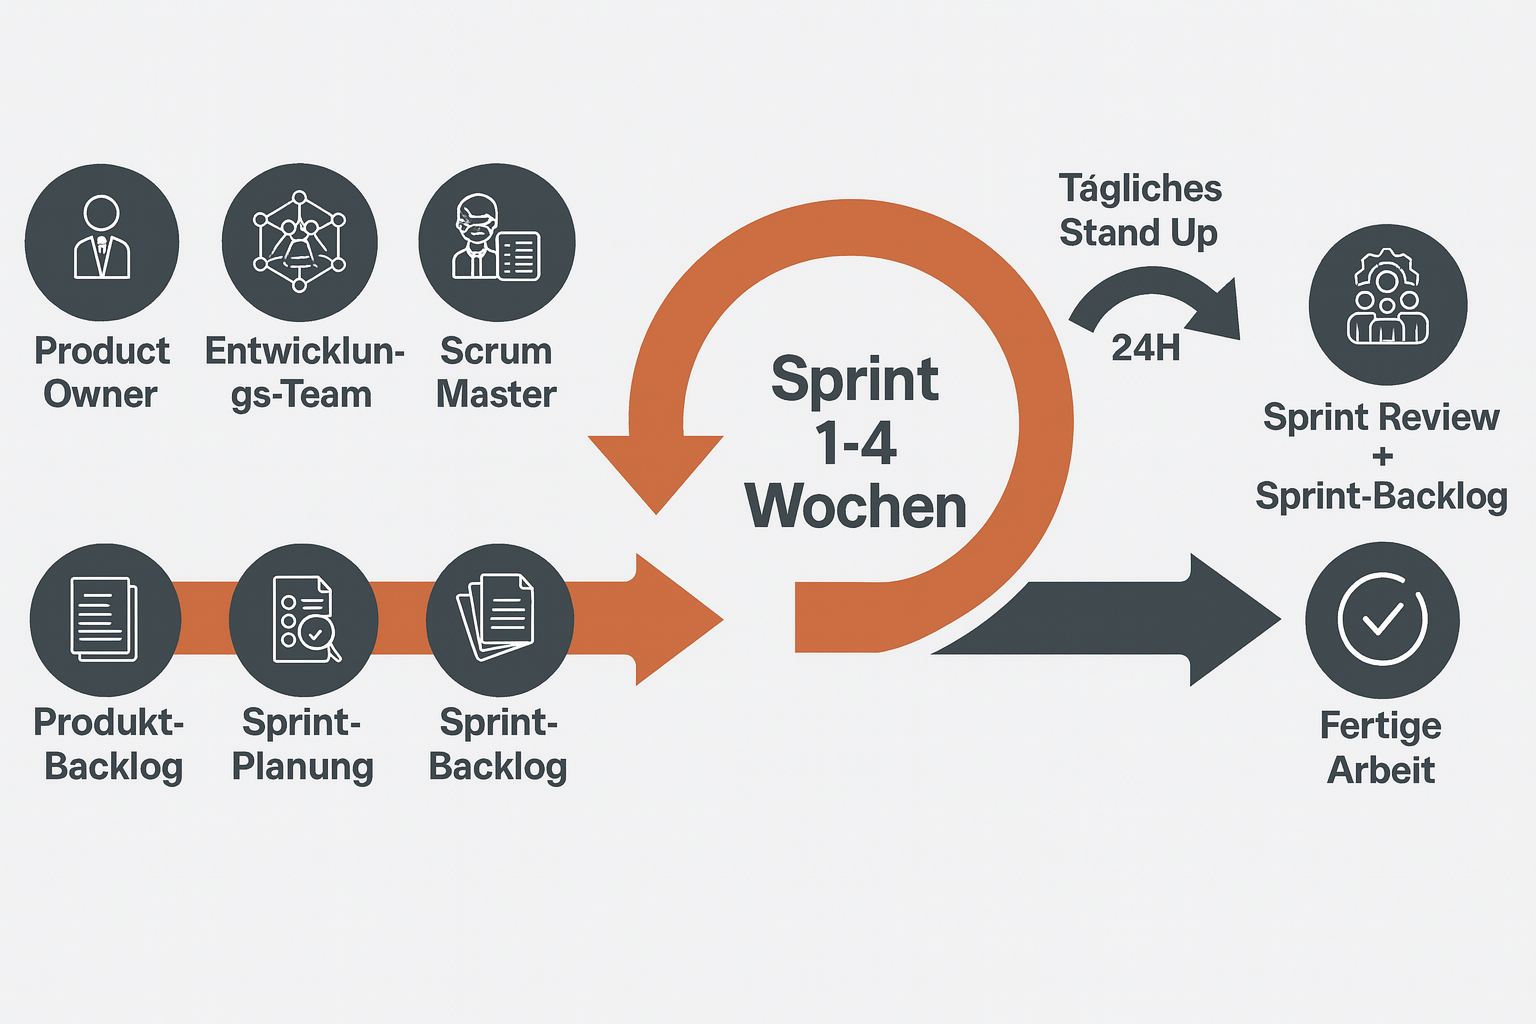
\includegraphics[width=0.5\linewidth]{images/scrum_ablauf.png}
    \caption{Ablauf eines typischen Scrum Sprints}
    \label{fig:scrum_ablauf}
\end{figure}
\end{document}
